\documentclass[crop, tikz]{standalone}

\usepackage{tikz}
\usepackage{amsmath}
\usepackage{amssymb}
\usepackage[mode=buildnew]{standalone}

\usepackage{xcolor}


\usetikzlibrary{fit}

\definecolor{mred}{RGB}{214,39,40}
\definecolor{mgreen}{RGB}{44,160,44}


\begin{document}
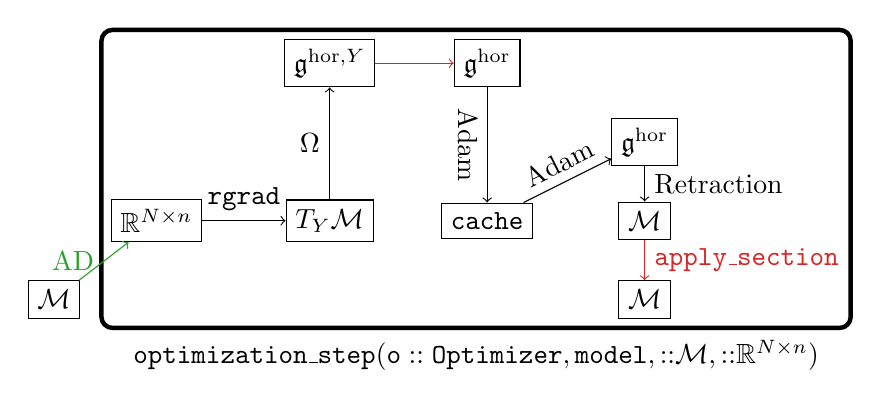
\begin{tikzpicture}
    \node[rectangle, draw] (TYM)   at (0, 0) {$T_Y\mathcal{M}$};
    \node[rectangle, draw] (ghorY) at (0, 2) {$\mathfrak{g}^{\mathrm{hor},Y}$};
    \node[rectangle, draw] (ghor)  at (2, 2) {$\mathfrak{g}^{\mathrm{hor}}$};
    \node[rectangle, draw] (cache) at (2, 0) {$\mathtt{cache}$};
    \node[rectangle, draw] (ghor2) at (4, 1) {$\mathfrak{g}^\mathrm{hor}$};
    \node[rectangle, draw] (M)	   at (4, 0) {$\mathcal{M}$};
    \node[rectangle, draw] (Euc)   at (-2.2,0) {$\mathbb{R}^{N\times{}n}$};
    \node[rectangle, draw] (M2)    at (-3.5,-1) {$\mathcal{M}$};
    \node[rectangle, draw] (M3)    at (4, -1) {$\mathcal{M}$};
    \coordinate[right of=M, xshift=1.5cm] (apply_section);
    \node[fit=(Euc)(ghorY)(ghor)(ghor2)(M3)(apply_section),draw, ultra thick, rounded corners, label=below:$\mathtt{optimization\_step(o::Optimizer,model, ::}\mathcal{M}\mathtt{,::}\mathbb{R}^{N\times{}n}\mathtt{)}$] (optimization_step) {};


    \draw[->] (TYM) -- (ghorY) node[pos=.5, left] {$\Omega$};
    \draw[->, mred] (ghorY) -- (ghor);
    \draw[->] (ghor) -- (cache) node[pos=.5, sloped, below] {Adam};
    \draw[->] (cache) -- (ghor2) node[pos=.5, sloped, above] {Adam};
    \draw[->] (ghor2) -- (M) node[pos=.5, right] {Retraction};
    \draw[->, mgreen] (M2) -- (Euc) node[pos=.5, left] {\color{mgreen}AD};
    \draw[->] (Euc) -- (TYM) node[pos=.5, above] {$\mathtt{rgrad}$};
    \draw[->, mred] (M) -- (M3) node[pos=.5, right] {$\mathtt{apply\_section}$};
\end{tikzpicture}
\end{document}